\chapter{СРАВНИТЕЛЬНЫЙ АНАЛИЗ АЛГОРИТМОВ}

\section{Постановка задачи}

Необходимо изучить и проанализировать существующие алгоритмы компьютерного зрения, провести практические эксперименты и впоследствии применить накопленные знания для решения задачи навигации беспилотного летательного аппарата в условиях отсутствия GPS.

Задачу навигации можно разбить на этапы:
\begin{enumerate}
    \item Построение 3D карты местности:
        \begin{itemize}
            \item сбор и подготовка данных;
            \item восстановление модели местности;
         \end{itemize}
    \item Разработка алгоритма навигации по существующей карте:
         \begin{itemize}
            \item нахождение себя на 3D карте по снимку;
            \item извлечение gps координат.
            \item осуществление навигации.
         \end{itemize}
    \item Оптимизация алгоритма для возможности построения карты в режиме реального времени на борту БПЛА.
\end{enumerate}

\section{Актуальность и практическая значимость}

Как следует из названия БПЛА не имеют пилота, но это не значит, что они не пилотируемы. Управление беспилотником требует специального обучения, сосредоточенности и является очень утомительным для оператора. Основополагающим необходимым условиям для работы дрона является наличие GPS сигнала, что делает его очень уязвимым и зависимым от внешних обстоятельств. В отсутствие сигнала системы глобального позиционирования дрон теряет управление.

В связи с этим возникает задача нахождения и использования альтернативных источников навигации. Так как почти каждый современный беспилотник оснащён камерой возможно применение алгоритмов компьютерного зрения.

С помощью разработанного алгоритма и программного обеспечения будет возможна навигация дрона, используя только камеру. Дополнительные возможности применения обширны: патрулирование заданной территории и обнаружение новых объектов, не присутствовавших ранее, возвращение в заданную точку в случае потери gps сигнала, слежение за данным объектом, навигация по заданной графической точке.

\section{Общие теоретические положения}   

Люди обладают зрением, что позволяет нам распознавать изображения и объекты на них, сравнивать их между собой и всё это мы делаем бессознательно, автоматически. Однако, для машины изображение — всего лишь закодированные данные, набор нулей и единиц. Одной из больших проблем в сопоставлении изображений является очень большая размерность пространства, которое несёт информацию. Если взять картинку размером хотя бы $100*100$ пикселей, то уже получим размерность равную $10^4$ пикселей. Поэтому методы анализа изображения должны быть быстрыми и эффективными. 

Как же компьютер обретает зрение? 

Основная идея состоит в том, чтобы получить какую-то характеристику, которая будет хорошо описывать изображение, легко вычисляться и для которой можно ввести оператор сравнения. Эта \quotes{характеристика} должна быть устойчива к различным преобразованиям (сдвиг, поворот и масштабирование изображения, изменения яркости, изменения положения камеры). Чтобы определять один и тот же объект на изображениях сделанных с разных углов, расстояний и при разном освещении.

Все эти условия приводят к необходимости выделения на изображении особых, \textit{ключевых точек} (\textbf{key points}). Этот процесс называется \textit{извлечение признаков} (\textbf{feature extraction}). Ключевая точка - эта такая особая точка, которая сильно отличается от близлежащих точек по какой-то обусловленной характеристике. Она должна быть не похожа на остальные точки вокруг, соответственно является, в какой-то степени, уникальным свойством изображения в своей локальной области. Таким образом машина может представить изображение как модель, состоящую из особых точек. Например, на изображении человеческого лица функции ключевых точек могут выполнять глаза, уголки губ, кончик носа.

После выделения особых точек компьютеру нужно уметь их сравнивать. Этот процесс называется \textit{сопоставление признаков} (\textbf{feature matching}). Для сравнения удобно использовать \textit{дескрипторы} (\textbf{descriptor} \quotes{описатель}). Дескриптор - своеобразный описатель или идентификатор ключевой точки, представляющий точку в удобном для сравнения виде. Как мы увидим далее, именно благодаря дескрипторам получается инвариантность относительно преобразований изображений. 
В итоге получается следующая схема решения задачи сопоставления изображений:

\begin{enumerate}
    \item Выделение ключевых точек и дескрипторов;
    \item Сравнение дескрипторов и нахождение паросочетаний соответствующий друг другу особых точек;
    \item Нахождение геометрического преобразования, которое переводит ключевые точки одного изображения в соответствующие им точки другого изображения.
\end{enumerate}

\begin{figure}[h]
    \centering
    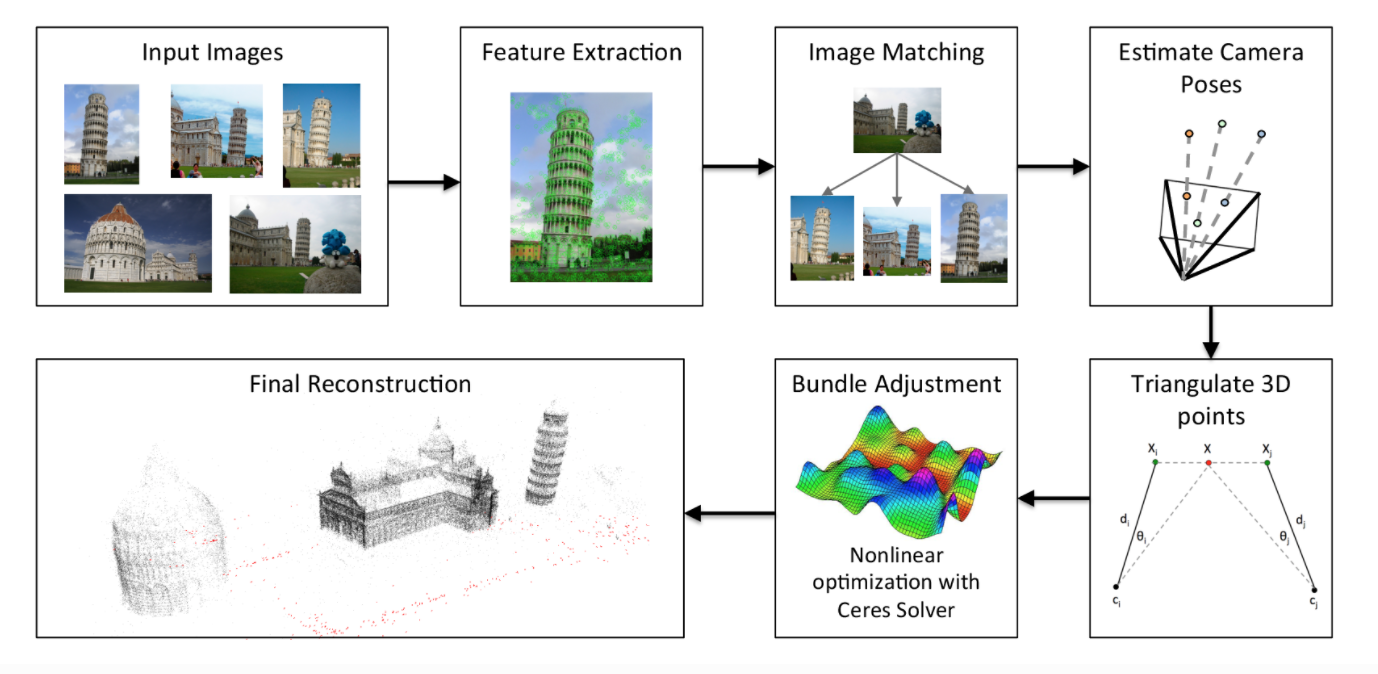
\includegraphics[width=1\textwidth]{sfm.png}
    \caption{\textbf{Structure From Motion}}
    \label{fig:sfm}
\end{figure}

На рисунке \ref{fig:sfm} представлена схема, демонстрирущая процесс извлечения \textit{структуры из движения} (\textbf{structure from motion}). Таким образом восстанавливается 3d модель поверхности.

Далее будут подробнее рассмотрены \textit{алгоритмы основанные на особых точках} (\textbf{feature-based algorithms}).

\section{Алгоритм SIFT}   

\textbf{Scale-invariant feature transform} (SIFT) - алгоритм компьютерного зрения для выделения ключевых точек и их дескрипторов. Алгоритм был разработан в Университете Британской Колумбии и опубликован Дэвидом Лоу (\textit{David G. Lowe}) в 1999 \hyperref[itm:lowe]{[\ref{itm:lowe}]}.
    
На первом этапе часто производится предварительная обработка изображения в целях улучшения его качества для последующего анализа. Например, на фотографиях с камер возможно появление шумов. Чтобы их устранить используют гауссовское размытие с маленьким радиусом или медианные фильтры.

\subsection{Извлечение ключевых точек}

Основополагающим моментом в нахождении особых точек является построение пирамиды гауссианов (\textbf{Gaussian}) и разностей гауссианов (\textbf{Difference of Gaussian, DoG}). Гауссианом (или изображением, размытым гауссовым фильтром) является изображение:
\begin{equation} \label{eq:1}
    L(x,y,\sigma) = G(x,y,\sigma) * I(x,y)
\end{equation} 

В уравнении (\ref{eq:1}): $L$ — значение гауссиана в точке с координатами $(x,y)$, а $\sigma$ — радиус размытия. $G$ — гауссово ядро, $I$ — значение исходного изображения, $*$ — операция свертки.

Разностью гауссианов называют изображение, полученное путем попиксельного вычитания одного гауссина исходного изображения из гауссиана с другим радиусом размытия:
\begin{equation} \label{eq:2}
    D(x,y,\sigma) = (G(x,y,k\sigma)-G(x,y,\sigma)) * I(x,y) = L(x,y,k\sigma) - L(x,y,\sigma)
\end{equation}

Таким образом, с помощью (\ref{eq:1}), мы получаем набор изображений, являющихся исходным изображением взятым в разных масштабах. Извлечение ключевых точке на определённом изображении из этого набора будет гарантировать инвариантность относительно сдвига, поворота и изменения размера изображения.

Как же выбирается нужный масштаб исходного снимка?. Для этого строится пирамида гауссианов (Рисунок \ref{fig:dog1}): весь набор масштабированных изображений разбивается на некоторые участки - октавы и при переходе от одной октавы к другой размеры изображения уменьшаются вдвое. После этого строится пирамида разностей гауссианов, состоящая из разностей соседних изображений в пирамиде гауссианов.

\begin{figure}[h]
    \centering
    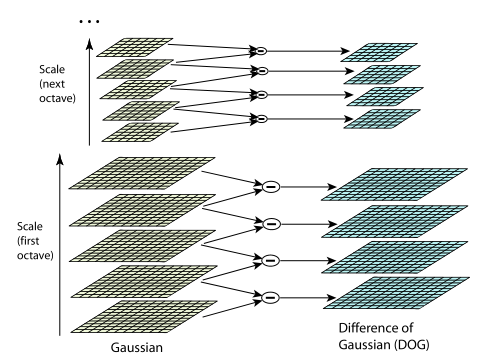
\includegraphics[width=0.6\textwidth]{dog.png}
    \caption{Пирамида гаусианнов}
    \label{fig:dog1}
\end{figure}

После построения пирамиды разностей гауссианов по всем точкам в пирамиде ищутся локальные экстремумы. Если точка больше (меньше) всех своих 26 соседей (Рисунок \ref{fig:dog2}) в пирамиде разностей, то она считается ключевой.

\begin{figure}[h]
    \centering
    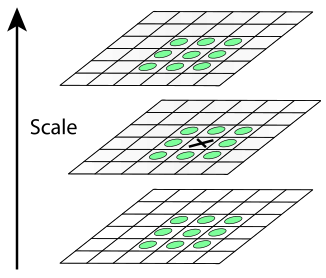
\includegraphics[width=0.5\textwidth]{dog2.png}
    \caption{Локальный экстремум в пирамиде Гауссианов}
    \label{fig:dog2}
\end{figure}

Направление особой точки вычисляется на изображении из пирамиды гауссианов в масштабе, полученном на предыдущем шаге. Ориентация ключевой точки - суммарное направление градиентов точек, находящихся в  $\sigma$-окрестности особой точки. Каждая точка окрестности влияет на итоговое направление. Величина и направление градиента в точке $(x,y)$ вычисляются по формулам (\ref{eq:3}) и (\ref{eq:4}) соответственно.

\begin{equation} \label{eq:3}
    m(x,y)=\sqrt{(L(x+1,y) - L(x-1,y))^2 + (L(x,y+1) - L(x,y-1))^2}
\end{equation}

\begin{equation} \label{eq:4}
    \theta(x,y)=\arctan{\left(\frac{L(x,y+1) - L(x,y-1)}{L(x+1,y) - L(x-1,y)}\right)}
\end{equation}

Таким образом для исходных изображений разных размеров мы получили ключевые точки (и небольшую область возле них) одного и того же размера - это и даёт инвариантность относительно масштабирования. А с помощью ориентации особой точки достигается инвариантность относительно поворота.

\subsection{Извлечение дескрипторов}

Как уже говорилось ранее, дескриптор должен уникально описывать ключевую точку. В общем случае это может быть любой объект, который будет выполнять данные функции: быть удобным для сравнения и являться инвариантным относительно преобразований исходного изображения.

В алгоритме SIFT дескриптор представляется как вектор, содержащий информацию об окрестности ключевой точки. Дескриптор вычисляется на том же гауссиане, на котом получен оптимальный размер особой точки. Для достижения инвариантности относительно поворота изображения перед вычислением всю область ключевой точки поворачивают на угол направления ключевой точки.

\begin{figure}[h]
    \centering
    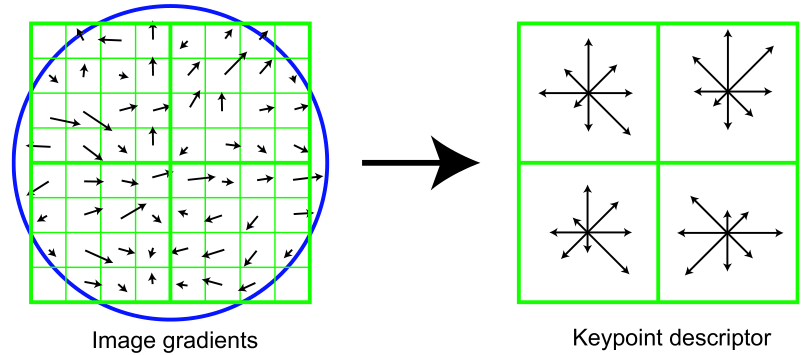
\includegraphics[width=0.8\textwidth]{desc.png}
    \caption{Получение дескриптора}
    \label{fig:desc}
\end{figure}

На Рисунке \ref{fig:desc} показана окрестность ключевой точки (слева) и построенный для неё дескриптор, состоящий из гистограмм (справа). Стрелочками в центре каждого пикселя в $\sigma$-окрестности обозначен градиент этого пикселя. Как видно на правой стороне изображения, дескриптор имеет размерность 2x2x8 (количество регионов по горизонтали, количество регионов по вертикали, количество компонент гистограммы этих регионов). Гистограмма для каждого региона является суммарным значением градиентов пикселей, входящих в $\sigma$-окрестность ($8$ штук).

Все полученные гистограммы и составляют итоговый дескриптор ключевой точки. В конце дескриптор нормализуется - все компоненты делятся на максимальное значение - в итоге каждая компонента находится в диапазоне $[0,1]$. Далее всем компонентам, значение которых больше $0.2$, присваивается значение $0.2$, а после этого дескриптор нормализуется ещё раз.

Как говорилось ранее, размер дескриптора равен 2x2x8 = $32$ компоненты, но на практике больше распространены и активнее используются дескрипторы размерности $128$ компонент (4x4x8).

\section{Анализ других алгоритмов}

SIFT дескрипторы не лишены недостатков. Не все полученные точки и их дескрипторы будут отвечать предъявляемым требованиям. Естественно это будет сказываться на дальнейшем решении задачи сопоставления изображений. В некоторых случаях решение может быть не найдено, даже если оно существует. Например, при поиске аффинных преобразований (или фундаментальной матрицы) по двум изображениям кирпичной стены может быть не найдено решения из-за того, что стена состоит из повторяющихся объектов (кирпичей), которые делают похожими между собой дескрипторы разных ключевых точек. Несмотря на это обстоятельство, данные дескрипторы хорошо работают во многих практически важных случаях. SIFT является наиболее математически обоснованным, но относительно медленным алгоритмом.

\subsection{Дескриптор SURF}

В 2008 был представлен ближайший конкурент SIFT дескриптора, \hyperref[itm:surf]{ SURF [\ref{itm:surf}]} дескриптор. В идейном смысле он похож на своего предшественника, но процедура описания окрестности особой точки несколько иная, поскольку в ней используются не гистограммы взвешенных градиентов, а отклики исходного изображения на \textit{вейвлеты Хаара} (\textbf{Haar wavelets}). Вейвлет — математическая функция, позволяющая анализировать различные частотные компоненты данных. Вейвлет Хаара — один из первых и наиболее простых вейвлетов, обладает компактным носителем, хорошо локализован в пространстве, но не является гладким. 

На первом шаге получения дескриптора вокруг ключевой точки строится квадратная область, которую ориентируют по некоторому предпочтительному направлению. Затем область разделяется на квадратные сектора. В каждом из секторов в точках, принадлежащих регулярной сетке, вычисляются отклики на два вида вейвлетов — горизонтально и вертикально направленные. Отклики взвешиваются Гауссианом, суммируются по каждому сектору, и образуют первую часть дескриптора.

Вторая часть дескриптора SURF состоит из сумм модулей откликов. Это сделано для того, чтобы учитывать не только факт изменения яркости от точки к точке, но и сохранить информацию о направлении изменения. SURF-дескриптор имеет длину 64. Как и SIFT, SURF-дескриптор инвариантен к аддитивному изменению яркости. Инвариантность к мультипликативному изменению яркости достигается путем нормировки дескриптора. SURF является эвристическим, но и более быстрым, чем SIFT.

\subsection{Дескриптор BRIEF}

Чем меньше длина дескриптора, тем меньше памяти требуется для его хранения, и меньше времени на сравнение его с другими. Эта черта очень важна при обработке большого числа изображений большой размерности. К наиболее компактным относится дескриптор \hyperref[itm:brief]{ BRIEF [\ref{itm:brief}]}. Для вычисления дескриптора в точке $p$ сравниваются значения яркости точек, расположенных в ее окрестности. При этом сравниваются значения яркости не всех точек со всеми, а анализируется лишь небольшое подмножество соседних пар точек, координаты которых распределены случайно (но одинаковым образом для каждой анализируемой точки $p$). Если яркость в точке $pi_1$ больше, чем яркость в точке $pi_2$, то $i$-я компонента дескриптора принимает значение $1$, в противном случае она становится равной нулю. Фрагмент, по которому вычисляются дескрипторы, предварительно сглаживается. BRIEF-дескрипторы чрезвычайно просты в вычислении, поскольку их значения равны результату сравнения двух чисел. Они также очень компактны, поскольку результат элементарного теста — это число $0$ или $1$, то есть один бит.

В стандартной реализации для построения одного BRIEF-дескриптора требуется выполнить $256$ сравнений, что дает итоговую длину $64$ байта. Это очень мало, учитывая, что SIFT-дескриптор состоит из $128$ действительных чисел, то есть занимает как минимум $512$ байтов. Наконец, сравнение BRIEF-дескрипторов занимает очень мало времени, поскольку сводится к вычислению \textit{расстояния Хэмминга} между двумя последовательностями битов. Расстояние Хэмминга (\textbf{Hamming distance}) — число позиций, в которых соответствующие символы двух слов одинаковой длины различны, вычисляется по формуле:

\begin{equation}
    d_{ij} = \sum_{k=1}^{p}|x_{ik} - x_{jk}|
\end{equation}

Эта элементарная операция выполняется чрезвычайно быстро на любом современном процессоре. Сами по себе дескрипторы BRIEF не инвариантны к повороту. Однако такой инвариантности можно добиться, если предварительно повернуть фрагмент вокруг ключевой точки на угол, соответствующий, например, доминирующему направлению градиента яркости, как это делается для дескрипторов SIFT и SURF. Точно так же можно достичь инвариантности к другим ракурсным искажениям.

\subsection{Дескриптор GLOH}

Дескриптор \hyperref[itm:gloh]{ GLOH (Gradient location-orientation histogram) [\ref{itm:gloh}]} является модификацией SIFT-дескриптора, который построен с целью повышения надежности. По факту вычисляется SIFT дескриптор, но используется полярная сетка разбиения окрестности на бины (Рисунок \ref{fig:gloh}): 3 радиальных блока с радиусами 6, 11 и 15 пикселей и 8 секторов. В результате получается вектор, содержащий 272 компоненты, который проецируется в пространство размерности 128 посредством использования анализа главных компонент.

\begin{figure}[h]
    \centering
    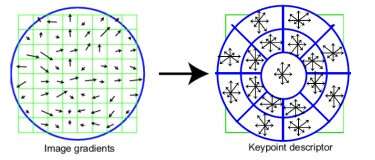
\includegraphics[width=0.8\textwidth]{gloh.jpg}
    \caption{Полярная сетка разбиения на бины}
    \label{fig:gloh}
\end{figure}

\subsection{FAST детектор}

FAST (Features from accelerated segment test - Особенности ускоренных испытаний сегмента) - алгоритм детекции ключевых точек. Детектор считает пиксели в круге Брезенгема (находится с помощью алгоритма Брезенгема построения кривых 2-го порядка) радиуса $r$ вокруг точки кандидата. Если n смежных пикселей ярче чем центр, по крайней мере, в $t$ раз или темнее центра, то пиксель под центром считается особенностью. Хотя r в принципе, может принимать любое значение, чаще всего используется значение $r=3$  (которому соответствует круг 16 пикселей окружности), и тесты показывают, что оптимальное значение $n=9$. Это значение n наименьшее, при котором края не обнаруживаются.

\subsection{Дескриптор ORB}

\hyperref[itm:orb]{ ORB (Oriented FAST and rotated BRIEF) [\ref{itm:orb}]} - ещё один алгоритм основанный на детекторе ключевых точек FAST и бинарных дескрипторах BRIEF. Как следует из названия, ORB дополняет и улучшает алгоритмы, на которых был основан. Алгоритм был предложен Ethan Rublee в 2010 году. Также как и BRIEF, ORB имеет размер 32 байта и для сравнения использует расстояния Хэмминга. После детектирования точек с помощью FAST-a ORB выделяет $N$ топ точек используя меру Харрисса. Далее ORB ориентирует найденные ключевые точки, что также отражено в его названии. Так как BRIEF плохо работает с поворотом, ORB исправляет это с помощью ориентации, полученной на предыдущем шаге.

\section{Выводы}

В этой главе мной были рассмотрены основные алгоритмы компьютерного зрения, с помощью которых можно находить и сравнивать ключевые точки. Подводя итог анализа: SIFT самый первый, математически точный и медленный дескриптор, на котором основаны большинство современных эвристических алгоритмов feature extraction. SURF - запатентованный в США алгоритм и поэтому является закрытым. Авторы BRIEF приводят результаты экспериментов в которых при одинаковых условиях на некоторых тестовых изображениях точность детектирования с помощью BRIEF почти в $1.5$ раза выше, чем с использованием SURF-дескрипторов. Дескриптор ORB быстрый, устойчивый ко многим искажениям и действительно является эффективной альтернативой алгоритму SIFT. Также ORB находится свободном доступе.

В своих дальнейших исследованиях я решил провести эксперименты с использованием SIFT - так как он является стандартом в компьютерном зрении, а ORB использовать как альтернативу и сравнить результаты по времени работы и точности сопоставления. OpenCV предоставляет удобный интерфейс создания дескрипторов и детекторов, что даёт возможность динамически сменять features methods. Практические эксперименты и их результаты будут рассмотрены в следующей главе.

\newpage